%This template (2020-03-06) is a modified version by Magnus Andersson and Jesper Erixon of the Stylish Article LaTeX Template Version 2.1 (1/10/15)
% Original author:
% Mathias Legrand (legrand.mathias@gmail.com) 
%
% License:
% CC BY-NC-SA 3.0

%----------------------------
\documentclass[fleqn,10pt]{SelfArx} % Document font size and equations flushed left
\usepackage[english]{babel} % Specify a different language here - English by default
\usepackage{lipsum} % Required to insert dummy text. To be removed otherwise
\usepackage{float} % Allow you to set the figure at a specific position, use mainly H 
% Additional packages
\usepackage{subcaption} % Allow you to create subfigures with individual captions
\usepackage{amsmath}
\usepackage{amssymb}
\usepackage{color}
\usepackage{graphicx}
\usepackage{float}
\usepackage{physics}
%\usepackage{hyperref}
\usepackage{caption}
%\usepackage{subcaption}
%----------------------------
%	COLUMNS
%----------------------------
\setlength{\columnsep}{0.55cm} % Distance between the two columns of text
\setlength{\fboxrule}{0.75pt} % Width of the border around the abstract
%----------------------------
%	COLORS
%----------------------------
\definecolor{color1}{RGB}{0,0,90} % Color of the article title and sections
\definecolor{color2}{RGB}{0,20,20} % Color of the boxes behind the abstract and headings
%----------------------------
%	HYPERLINKS
%----------------------------
\usepackage{hyperref} % Required for hyperlinks
\hypersetup{hidelinks,colorlinks,breaklinks=true,urlcolor=color2,citecolor=color1,linkcolor=color1,bookmarksopen=false,pdftitle={Title},pdfauthor={Author}}
\urlstyle{same} % Sets url font
\usepackage{cleveref} % Added: Use cleveref to be able to reference subfigures e.g. Fig 1(a) etc.
\captionsetup[subfigure]{subrefformat=simple,labelformat=simple} % Added: Setup subfigure label
\renewcommand\thesubfigure{(\alph{subfigure})}
%----------------------------
%	ARTICLE INFORMATION
%----------------------------
\JournalInfo{Department of Physics, Umeå University}
\Archive{\today}

\PaperTitle{Simulating the bistability of histone methylation.} % Article title

\Authors{Henrik Linder\textsuperscript{1}*} % Authors
\affiliation{\textsuperscript{1}\textit{Department of Physics, Umeå University, Umeå, Sweden}} % Author affiliation
\affiliation{*\textbf{Corresponding author}: heli0152@student.umu.se} % Corresponding author
\affiliation{*\textbf{Supervisor}: Lucas Hedström, lucas.hedstrom@umu.se}
\Keywords{DNA -- Methylation -- Epigenetics -- Bistability} % Keywords - if you don't want any simply remove all the text between the curly brackets
\newcommand{\keywordname}{Keywords} % Defines the keywords heading name
%----------------------------
%	ABSTRACT
%----------------------------
\Abstract{
	%The thin lens equation can predict how lenses in an optical system refract light. In this exercise, we investigated how well our theoretical predictions coincided with our experimental findings. \textcolor{red}{\textit{What was done?}} Using the thin lens equation, we first derived the distance to the image plane for an object positioned in front of a convex and concave lens and thereafter experimentally measured the distances. \textcolor{red}{\textit{How was it done?}} We found that the experiments agreed with the theoretical predictions, with a discrepancy of only 1.0 $\pm$ 0.2 mm. \textcolor{red}{\textit{What was found?}} We then built and verified the performance of both a Kepler and a Galilean telescope. We found that theory and experiment coincided with a discrepancy of 3.0 $\pm$ 0.3 mm. However, we observed a significant amount of aberrations, which we suggest is related to the spherical shaped lenses used in the setup. The findings in this exercise suggest that the thin lens equation can accurately predict how lenses should be positioned for imaging purposes, but that it does not take into account the degree of aberrations.\textcolor{red}{\textit{{What is the significance of the findings?.}}}
	DNA-methylation is a modification to the DNA-structure that can change the expression of the DNA without changing the gene sequence itself by adding methyl or acethyl groups. This is studied in this lab by simulating a few different models for the evolution of the methylation over time. We found that the ratio of active to noisy conversion between methylation states plays a vital role in the stability of the system. 
	By changing the way methylated nucleosomes are chosen, we found that it is important to have a non-linear dependency on methylation concentration in order to achieve a bistable system.
%
We also varied how the probability of active conversion depended on distance, and found that only local active conversion does not give rise to a bistable system. Lastly, we simulated cell division by randomly removing half of the methylation and found that the methylation state is remarkably stable even under cell division.
%Epigenetics is the study of how one may obtain different expression sfrom the same gene sequences. One epigenetic mechanism is DNA-methylation, where methyl or acethyl groups are added to the histones that make up the DNA nucleosomes. These methyl groups change the expression of the genes and are therefore interesting to study.
%The methylation of a gene sequence can change over time, and is affected both by random noise and by active conversion from nucleosomes nearby. The purpose of this lab is to study this change in methylation and determine the stability of the system, as well as finding out whether a methylated gene sequence can survive a cell division. 
}

%----------------------------
\begin{document}

\flushbottom % Makes all text pages the same height

\maketitle % Print the title and abstract box

\tableofcontents % Print the contents section

\thispagestyle{empty} % Removes page numbering from the first page

%----------------------------
%	ARTICLE CONTENTS
%----------------------------

%----------------------------


%\documentclass{article}
%\usepackage[utf8]{inputenc}
%\usepackage{amsmath}
%\usepackage{amssymb}
%\usepackage{color}
%\usepackage{graphicx}
%\usepackage{float}
%\usepackage{physics}
%\usepackage{hyperref}
%\usepackage{caption}
%\usepackage{subcaption}
%\title{report v0.tex }
%\author{Henrik Linder}
%\date{\today}
%\begin{document}
%\maketitle

%Wolfram alpha, eq 7.1 for a  : \href{https://www.wolframalpha.com/input?i=solve+0+\%3D+alpha*\%28a*\%281-a-m\%29+-+a*m\%29+\%2B+\%281+-+alpha\%29*\%28\%281-a-m\%29\%2F2+-+a\%29+for+a+}{here }
%Wolfram alpha, eq 7.1 for m  : \href{https://www.wolframalpha.com/input?i=solve+0+%3D+alpha*%28a*%281-a-m%29+-+a*m%29+%2B+%281+-+alpha%29*%28%281-a-m%29%2F2+-+a%29+for+m}{here }

%Solve eq 7.2 in steady state for a : \href{https://www.wolframalpha.com/input?i=solve+0+\%3D+alpha*\%28m*\%281-a-m\%29+-+a*m\%29+\%2B+\%281+-+alpha\%29*\%28\%281-a-m\%29\%2F2+-+a\%29+for+a+}{here}
%Solve eq 7.2 in steady state for m: \href{https://www.wolframalpha.com/input?i=solve+0+%3D+alpha*%28m*%281-a-m%29+-+a*m%29+%2B+%281+-+alpha%29*%28%281-a-m%29%2F2+-+a%29+for+m}{here}




%Steady state when both are zero: 

%for a=m : 
%\href{https://www.wolframalpha.com/input?i=solve+0+%3D+alpha*%28a*%281-a-a%29+-+a*a%29+%2B+%281+-+alpha%29*%28%281-a-a%29%2F2+-+a%29+for+a+}{sloution}

%equal to eachother: 
%\href{https://www.wolframalpha.com/input?i=solve+alpha*%28m*%281-a-m%29+-+a*m%29+%2B+%281+-+alpha%29*%28%281-a-m%29%2F2+-+m%29++%3D+alpha*%28a*%281-a-m%29+-+a*m%29+%2B+%281+-+alpha%29*%28%281-a-m%29%2F2+-+a%29+for+a+}{here}



%differentiation : 
%%[200~https://www.wolframalpha.com/input?i=differentiate+alpha*%28m*%281-a-m%29+-+a*m%29+%2B+%281+-+alpha%29*%28%281-a-m%29%2F2+-+m%29+with+respect+to++m]



%in task4\_nr\_methylated\_v2, and v3 i managed to get one to switch over 


\section{Introduction}
Epigenetics is the study of how one may obtain different expressions from the same gene sequences. One epigenetic mechanism is DNA-methylation, where methyl or acethyl groups are added to the histones that make up the DNA nucleosomes. These methyl groups change the expression of the genes and are therefore interesting to study.
The methylation of a gene sequence can change over time, and is affected both by random noise and by active conversion from nucleosomes nearby. The purpose of this lab is to study this change in methylation and determine the stability of the system, as well as finding out whether the methylation of a gene sequence can survive cell division. 

\section{Task 1: Standard model for yeast epigenetics}
%The expression of genes is determined not only by the 
\subsection{Theory}

A nucleosome can be in one of three methylation states: Methylated (M), Acethylated (A), or Unmethylated (U). 
The equations governing the change of methylation are the following

\begin{equation}
	\dv {a}{t} = f = \alpha[a(1-a-m) - am] + (1-\alpha )\left(\frac{1-a-m}{2}  - a\right)
	\label{eq:dadt}
\end{equation}
\begin{equation}
	\dv {m}{t} = g = \alpha[m(1-a-m) - am] + (1-\alpha )\left(\frac{1-a-m}{2}  - m\right),
	\label{eq:dmdt}
\end{equation}
where $a$ and $m$ are the fraction of nucleosomes in the A and M states, respectively. $\alpha$ is a parameter describing the probability of conversion.

In this lab we will mostly work instead with the parameter 
\begin{equation}
	F = \frac{\alpha}{1-\alpha}
	\label{eq:F}
\end{equation}
which defines the ratio of active to random conversions. 

\begin{figure*}[ht]
	\centering
	\begin{subfigure}[b]{.3\textwidth}
		\centering
		\includegraphics[width= \linewidth]{figs2/task1_F2_v4.eps}
		\caption{F = 2}
		\label{fig:task1_F2}
	\end{subfigure}
	\begin{subfigure}[b]{.3\textwidth}
		\centering
		\includegraphics[width= \linewidth]{figs2/task1_F4_v4.eps}
		\caption{F = 4}
		\label{fig:task1_F4}
	\end{subfigure}
	\begin{subfigure}[b]{.3\textwidth}
		\centering
		\includegraphics[width= \linewidth]{figs2/task1_F6_v8.png}
		\caption{F = 6}
		\label{fig:task1_F6}
	\end{subfigure}
	\begin{subfigure}[b]{.3\textwidth}
		\centering
		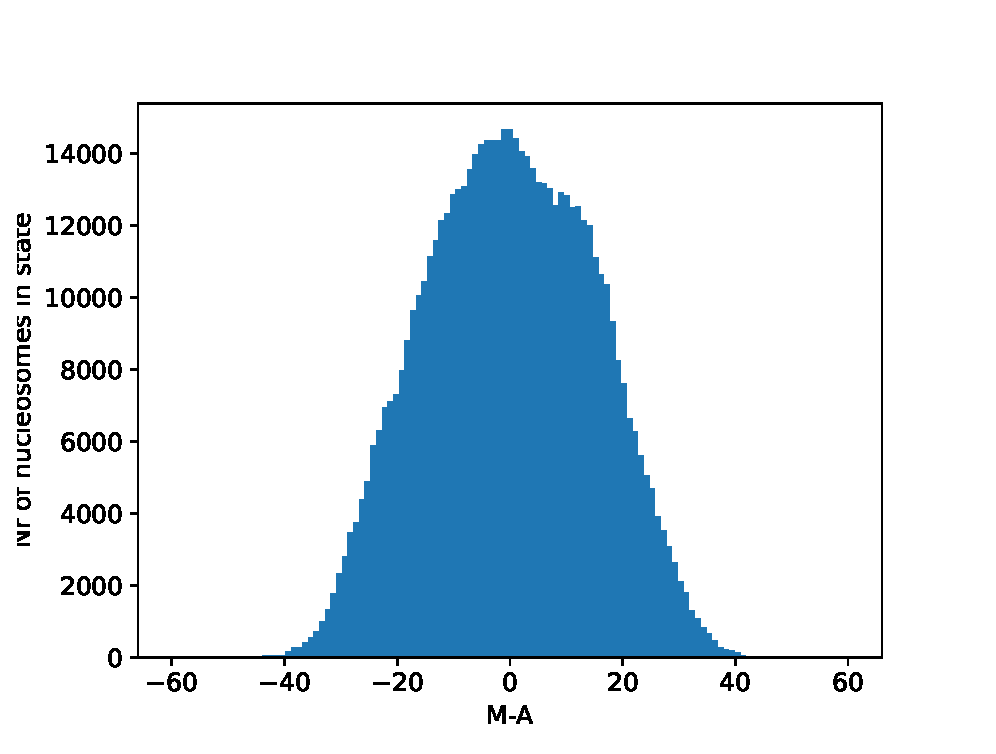
\includegraphics[width= \linewidth]{figs2/task1_F2_hist_v4.eps}
		\caption{F = 2}
		\label{fig:task1_F2_hist}
	\end{subfigure}
	\begin{subfigure}[b]{.3\textwidth}
		\centering
		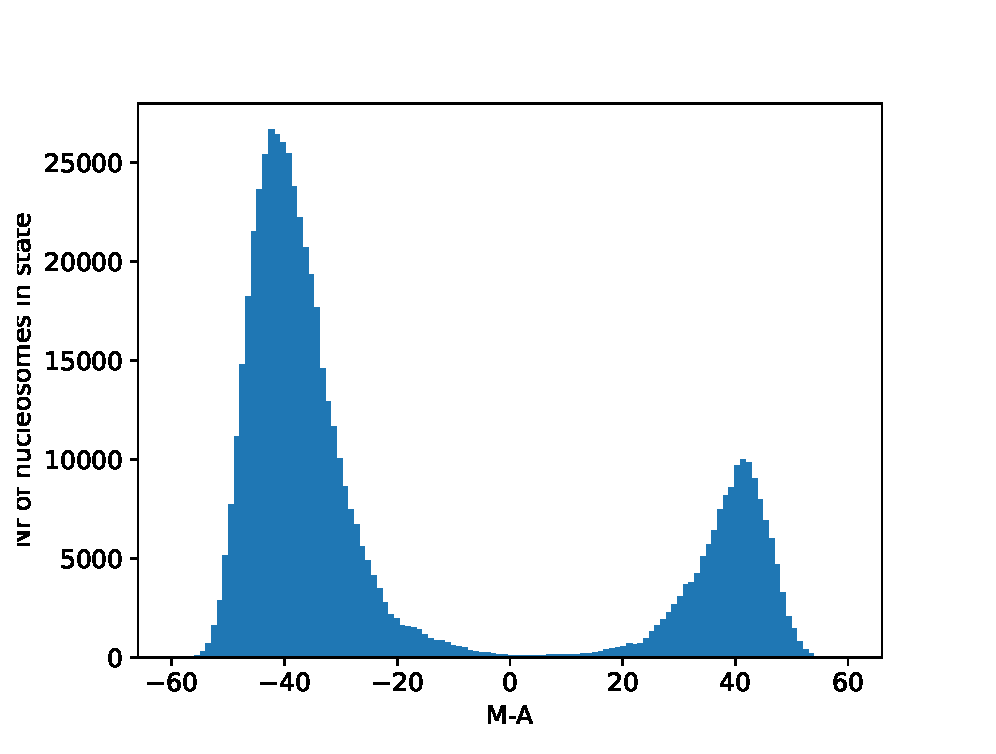
\includegraphics[width= \linewidth]{figs2/task1_F4_hist_v4.eps}
		\caption{F = 4}
		\label{fig:task1_F4_hist}
	\end{subfigure}
	\begin{subfigure}[b]{.3\textwidth}
		\centering
		\includegraphics[width= \linewidth]{figs2/task1_F6_hist_v5.eps}
		\caption{F = 6}
		\label{fig:task1_F6_hist}
	\end{subfigure}
		\caption{The top row shows the number of nucleosomes in the M state versus time for different values of F. The bottom row shows a histogram of the number of histones in the M and A states throughout the entire simulation. }
		\label{fig:task1}
\end{figure*}

Solving eqs \eqref{eq:dadt} and \eqref{eq:dmdt} in steady state for $m=a$, we get 
\begin{equation}
	m = \frac{\sqrt{3\alpha^2 - 6\alpha + 4} + 3\alpha - 2}{6\alpha}.
	\label{eq:m_of_alpha}
\end{equation}
where we for alpha will use 
\begin{equation}
	\alpha = \frac{F}{1 + F}.
\label{eq:alpha_of_F}
\end{equation}


Sneppen \cite{book} gives us that the stability of a fixed point is determined by the sign of the largest eigenvalue, given by the following equation
\begin{equation}
	\lambda = \frac{f_a + g_m}{2}  + \sqrt{\frac{\left(f_a + g_m\right)^2}{4} - f_ag_m + f_mg_a},
	\label{eq:eigen}
\end{equation}
where
\begin{equation}
	f_a = \dv{f}{a},\quad
	g_a = \dv{g}{a},\quad
	f_m = \dv{f}{m},\quad
	g_m = \dv{g}{m}.
\end{equation}

These derivatives were all found using the symbolic solver Wolfram Alpha \cite{wolfram}. 

Now we can substitute these derivatives and eqs \eqref{eq:alpha_of_F} and \eqref{eq:m_of_alpha} into eq.\eqref{eq:eigen} to get the eigenvalue as a function of $F$. Now we plug $\lambda = 0$ into wolfram alpha \cite{wolfram} and solve for $F$ to get the $F$ at which the eigenvalue switches sign. This yields that the critical point at which the system goes from stable to bistable is at
\begin{equation}
	F_c = \frac{1}{\sqrt{2} - 1}.
\end{equation}


\subsection{Results and discussion}
$F$ increasing means that the ratio of active recruitment to random conversion between M and A states increases. This means that at high values of F, it is much more likely that a nucleosome is changed by conversion from another nucleosome than by random noise. As random chance has less and less effect, the bistability becomes more pronounced. In the limit, as $F\to\infty$, the noise will become negligible and the system will tend to end up in a state of only A or M, and stay that way indefinitely. 

In the other limit, as $F\to 0$, the noise dominates and the effect of recruitment becomes negligible. The evolution of the system then becomes a random walk. 

This progression is seen in fig.\eqref{fig:task1}. Starting from $F=2$, the methylation is essentially random in fig.\eqref{fig:task1_F2}, giving rise to the single normal distribution around $M-A=0$ in the histogram in fig.\eqref{fig:task1_F2_hist}. When $F=4$, the system displays a pronounced bistability, jumping from high methylation to high acethylation in fig.\eqref{fig:task1_F4}, giving rise to the twin peaks in fig.\eqref{fig:task1_F6_hist}. Going as far as $F=6$, the system is very stable for very long periods of time, shown in fig.\eqref{fig:task1_F6}, resulting in the narrow twin peaks in fig.\eqref{fig:task1_F6_hist}.


\begin{figure*}[ht!]
	\centering
	\begin{subfigure}[t]{.49\textwidth}
		\centering
		\includegraphics[width= \linewidth]{figs2/task2_m_vs_t_v1.eps}
		\caption{Nr of methylated nucleosomes versus time. }
		\label{fig:task2_m_vs_t}
	\end{subfigure}
	\begin{subfigure}[t]{.49\textwidth}
		\centering
		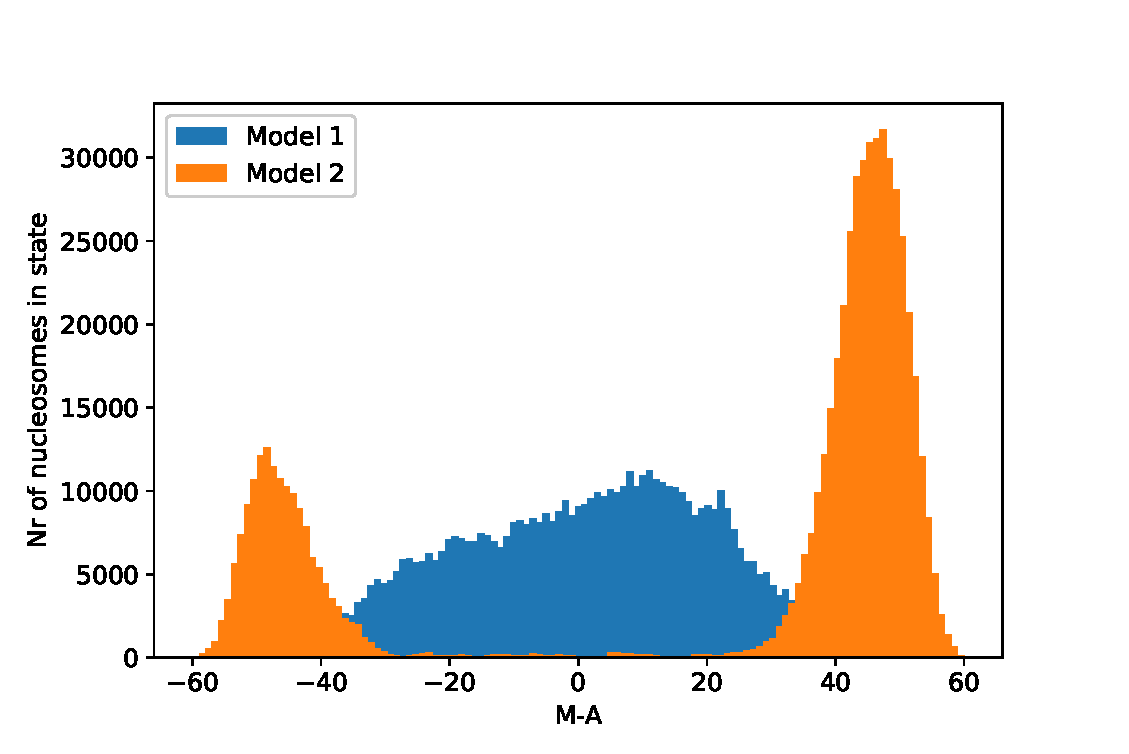
\includegraphics[width= \linewidth]{figs2/task2_hist_v1.eps}
		\caption{Histogram showing the distribution of methylation states over the simulation.}
		\label{fig:task2_hist}
	\end{subfigure}
		\caption{The results of simulations in task 2 with both model 1 and model 2, having linear and non-linear dependencies on $m$, respectively.}
		\label{fig:task2}
\end{figure*}




\section{Task 2: Epigenetics and cooperativity}
\subsection{Theory}
We will call the model in the previous task model 0. In order to study the effects of non-linerarity on the bistability of the system, we remove one of the active recruitment steps from the model to obtain the equations below which we call 
model 1
\begin{equation}
	\dv {a}{t} = f = \alpha[a(1-a-m)] + (1-\alpha )\left(\frac{1-a-m}{2}  - a\right)
\end{equation}
\begin{equation}
	\dv {m}{t} = g = \alpha[m(1-a-m)] + (1-\alpha )\left(\frac{1-a-m}{2}  - m\right).
\end{equation}
Here, we only require interaction with a single nucleosome for active recruitment, going from the U state. Going from an A or M state to a U state can only be done through noisy conversion. 

If we do a similar stability analysis as for the previous model, we find that there are no fix points for this model for $m\neq a$ and when $m=a$, the fix points are unstable. 
%source:https://www.wolframalpha.com/input?i=solve+alpha*%28m*%281-a-m%29%29+%2B+%281+-+alpha%29*%28%281-a-m%29%2F2+-+m%29%3Dalpha*%28a*%281-a-m%29%29+%2B+%281+-+alpha%29*%28%281-a-m%29%2F2+-+a%29++%3D0+for+m+


For model 2 below, we add back the non-linearity by requiring two random nucleosomes with the same methylation be chosen in order to convert a nucleosome from a U state. 
%source: https://www.wolframalpha.com/input?i=solve+alpha*%28m%5E2*%281-a-m%29%29+%2B+%281+-+alpha%29*%28%281-a-m%29%2F2+-+m%29%3Dalpha*%28a%5E2*%281-a-m%29%29+%2B+%281+-+alpha%29*%28%281-a-m%29%2F2+-+a%29++%3D0+for+m+
\begin{equation}
	\dv {a}{t} = f = \alpha[a^2(1-a-m)] + (1-\alpha )\left(\frac{1-a-m}{2}  - a\right)
\end{equation}
\begin{equation}
	\dv {m}{t} = g = \alpha[m^2(1-a-m)] + (1-\alpha )\left(\frac{1-a-m}{2}  - m\right)
\end{equation}


\subsection{Results and discussion}
In order for bistability to occur, we need a non-linear feedback loop. This is achieved in model 0 by requiring two separate nucleosomes for a full conversion to occur. However, in model 1, we only require one, meaning that the conversion only depends linearly on the concentration of A or M. This shows in the fact that the results in this task display no (or at least very little) bistable behavior, despite working at an $F$ that would have been distinctly bistable in the previous model. 

We can add back the non-linearity into the model by requiring two random nucleosomes of the same methylation be picked in order to convert an unmethylated nucleosome into an A or M state. Now the active recruitment once again depend on the square of the concentration of M, so we get the bistable behavior similar to that of the first model. 

The difference is clearly shown in fig. \eqref{fig:task2} where we can see clear bistable behavior in model 2, while model 1 appears to be doing a random walk. 


\begin{figure*}[ht!]
	\centering
	\begin{subfigure}[b]{.49\textwidth}
		\centering
		\includegraphics[width= \linewidth]{figs2/task3_2_2_v0.eps}
		\caption{Nr of methylated nucleosomes versus time for $\gamma=2.2$ }
		\label{fig:task3_m_vs_t_2_2}
	\end{subfigure}
	\begin{subfigure}[b]{.49\textwidth}
		\centering
		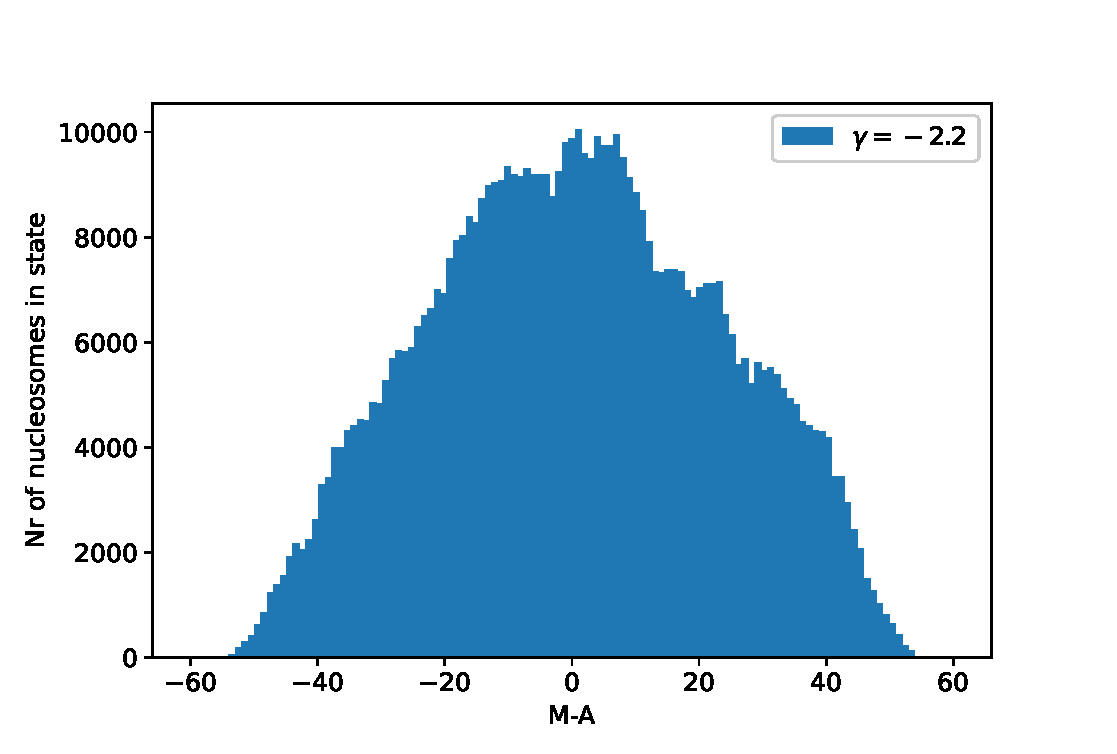
\includegraphics[width= \linewidth]{figs2/task3_hist_2_2_v0.eps}
		\caption{Histogram showing the distribution of methylation states over the simulation for $\gamma=2.2$.}
		\label{fig:task3_hist_2_2}
	\end{subfigure}
	\begin{subfigure}[b]{.49\textwidth}
		\centering
		\includegraphics[width= \linewidth]{figs2/task3_1_8_v0.eps}
		\caption{Nr of methylated nucleosomes versus time for $\gamma=1.8$.}
		\label{fig:task3_m_vs_t_1_8}
	\end{subfigure}
	\begin{subfigure}[b]{.49\textwidth}
		\centering
		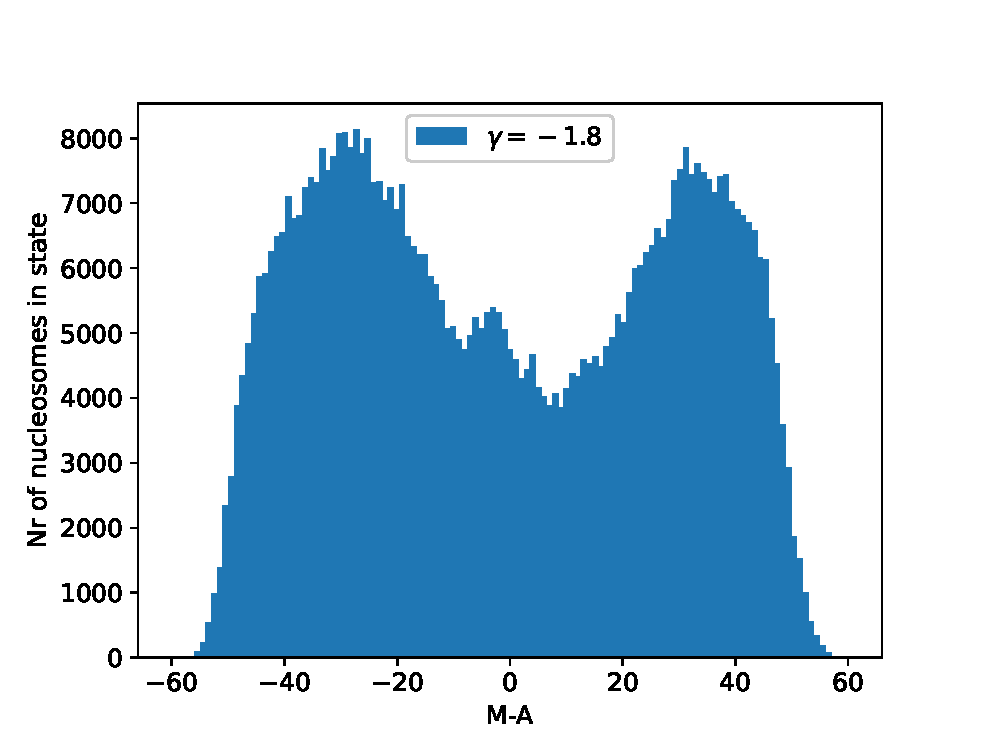
\includegraphics[width= \linewidth]{figs2/task3_hist_1_8_v0.eps}
		\caption{Histogram showing the distribution of methylation states over the simulation for $\gamma=1.8$.}
		\label{fig:task3_hist_1_8}
	\end{subfigure}
	\begin{subfigure}[b]{.49\textwidth}
		\centering
		\includegraphics[width= \linewidth]{figs2/task3_1_4_v0.eps}
		\caption{Nr of methylated nucleosomes versus time for $\gamma=1.4$.}
		\label{fig:task3_m_vs_t_1_4}
	\end{subfigure}
	\begin{subfigure}[b]{.49\textwidth}
		\centering
		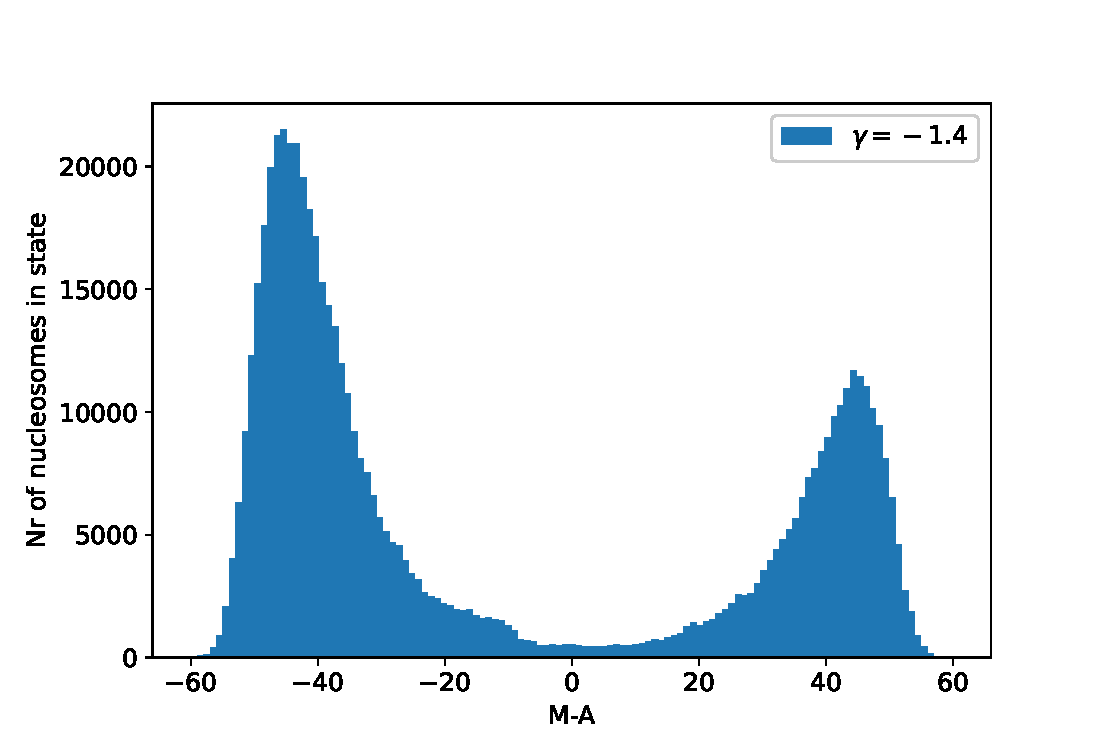
\includegraphics[width= \linewidth]{figs2/task3_hist_1_4_v0.eps}
		\caption{Histogram showing the distribution of methylation states over the simulation for $\gamma=1.4$.}
		\label{fig:task3_hist_1_4}
	\end{subfigure}
		\caption{The result for simulations in task 3, showing the methylation for different values of $\gamma$. On the left is how the number of methylated histones change over time in each simulation, and on the right are histograms showing the distribution of methylation states over the entire run time of the simulation. From the top down, this is shown for the values of $\gamma = {-2.2, -1.8, -1.4}$.}
		\label{fig:task3}
\end{figure*}
\begin{figure*}[ht!]
	\centering
	\begin{subfigure}[b]{.49\textwidth}
		\centering
		\includegraphics[width= \linewidth]{figs2/task4_m_vs_t_v0.eps}
		\caption{Nr of methylated nucleosomes versus time. The time of cell divisions is marked with red lines. }
		\label{fig:task4_m_vs_t}
	\end{subfigure}
	\begin{subfigure}[b]{.49\textwidth}
		\centering
		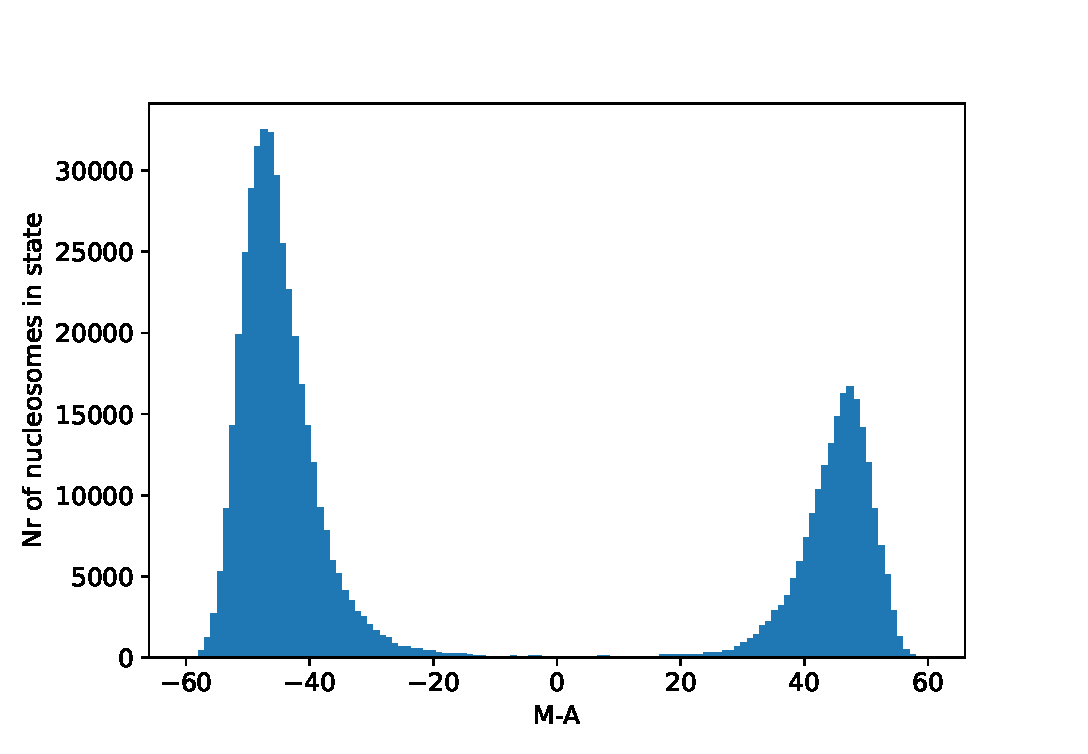
\includegraphics[width= \linewidth]{figs2/task4_hist_v0.eps}
		\caption{Histogram showing the distribution of methylation states over the simulation.}
		\label{fig:task4_hist}
	\end{subfigure}
		\caption{The results of simulations in task 4 with ten cell divisions occuring during the run of the simulation. }
		\label{fig:task4}
\end{figure*}

\section{Task 3: Local vs. non-local interactions}
\subsection{Theory}
In the previous models, we have assumed that every nucleosome has an equal chance of converting every other nucleosome, regardless of their respective placement on the chain of nucleosomes. 

It stands to reason that the distance between nucleosomes may affect the probability of them interacting, so we will incorporate a dependency on distance in the recruitment probability. The new probability of interaction between two nucleosomes will decay like 
%This may not 
\begin{equation}
	P(d) \propto d^\gamma
\end{equation}
where $d$ is the distance between two nucleosomes, and $\gamma <0$ is some parameter. In these simulations, 
we use $\gamma\in [-1,-3]$. 
\subsection{Results and discussion}



$\gamma$ is a constant determining the rate at which the recruitment probability decays with the distance along the nucleosome chain. As $\gamma$ decreases, the probability decays faster and faster, until the recruitment process is entirely local. A local recruitment mechanism does not display a bistable behavior, while a global -- as shown by model 0-- does. 

In model 0, there was no distance dependency, recruitment was equally likely from every other nucleosome in the chain. This model is therefore entirely global. 
This is the baseline to which we can compare the behavior of the new model. 
As $\gamma\to 0$, the probability vector becomes uniform (does not decay with distance), and the result is the same as in model 0.

As expected from this reasoning, the lower values of $\gamma$ do not give rise to a bistable behavior in the system, while the higher do. 

The cut-off value of $\gamma$ seem to be just below 2, as indicated by fig.\eqref{fig:task3}. 
Here we can see the system displaying clear bistability at $\gamma = 1.4$, and none at all at $\gamma= 2.2$. $\gamma= 1.8$ seems to be in the transitional region between the two, indicating that $\gamma$ just under two is the limit if we want our system to behave bistably. 








\section{Task 4: Can epigenetic states survive cell division?}
\subsection{Theory}
In the previous tasks, we have shown that the epigenetic modifications can be quite stable under certain circumstances. But can they be transferred to a daughter cell through cell division?
During cell division, there is a probability of 0.5 that the methylated nucleosome will end up in each of the new DNA strings. In the other DNA string, this nucleosome will be replaced by an unmethylated nucleosome. 
In this task, we simulate this cell division by changing each nucleosome to unmethylated with a probability of 0.5.
As a base, we use model 0 from the first task with $F=6$.
\subsection{Results and discussion}

As shown by fig.\eqref{fig:task4}
%\textcolor{red}{FIGURE HERE}
, the system will tend to keep its methylation state throughout cell division, although there is a heightened chance of the noise conversion tipping the system over to the opposite methylation state. 


In fig.\eqref{fig:task4_m_vs_t}
%\textcolor{red}{ fig  } 
we can see that the number of metylated nucleosomes dip during cell division, but quickly recover as they are recruited from the unmethylated state by the methylated nucleosomes. However, as this is a stochastic process with a significant noise component, the probability of switching over to the other stable methylation state is significantly higher right after cell division. 

This make sense since the absolute number of nucleosomes affected will be greater for the dominant state, bringing the system closer to the unstable fixed point where it is more likely to be tipped over by the random noise conversion. 

Compare this to the corresponding simulation in task 1 (model 0, $F=6$), where it was found that there was essentially no chance (at this $F$) of switching between an acethyl-dominated and a methyl-dominated state on these time scales. 

%It is still an impressive stability, being able to keep the methylation state when removing half of all methyl or acethyl groups. 
That said, it is still quite stable. The system keeps its methylation during cell division in the majority of cases, indicating that it may well be able to transfer epigenetic information across generations.
 


\begin{thebibliography}{3}
\bibitem{book}
Sneppen, K. \textit{Models of life -- Dynamics and regulation in biological systems.} (Cambridge University Press, 2014)
\bibitem{wolfram}
\href{Wolframalpha.com}{Wolframalpha.com}
\end{thebibliography}






\end{document}
